\documentclass[answers]{exam}
\usepackage[utf8]{inputenc}

\usepackage[dvipsnames]{xcolor}
\usepackage{amsmath}
\usepackage{amsfonts}
\usepackage{amsthm}
\usepackage{microtype}
\usepackage{siunitx}
\DeclareSIUnit\year{yr}
\usepackage{pgfplots}
\usepackage{graphicx}
\usepackage{sidecap}
\sidecaptionvpos{figure}{c}
\usepackage{float}
\usepackage{gensymb}
\usepackage{tkz-euclide}
\usetkzobj{all}
\usepackage{commath}
\usepackage{hyperref}
\usepackage{enumitem}
\usepackage{wasysym}
\usepackage[parfill]{parskip}

\renewcommand*{\thefootnote}{\fnsymbol{footnote}}

\newtheorem*{thm}{Theorem}
\newtheorem*{iden}{Identity}
\newtheorem*{lemma}{Lemma}
\theoremstyle{definition}
\newtheorem*{defn}{Definition}
\newtheorem*{ex}{Example}

% russian integral
\usepackage{scalerel}
\DeclareMathOperator*{\rint}{\scalerel*{\rotatebox{17}{$\!\int\!$}}{\int}}

% \qformat{Question \thequestion: \thequestiontitle\hfill}

\begin{document}

\section*{NCEA Level 3 Physics (Modern Physics)}
A nucleus is what is known as a \textit{bound system}. In other words, energy must be supplied
in order to break the bonds between the nucleons. This is similar to the way that electrons
orbiting the nucleus are in negative energy levels --- we supply the ionization energy to free
the electrons from the bound system.

The energy which must be supplied to the nucleus to break it apart is known as the \textit{binding
energy}, and is on the order of tens or hundreds of \si{\mega\electronvolt}. This amount is high
enough that its mass equivalence is non-negligible.

Consider some nucleus $ ^w_nX $ with a mass $ M $. Experimentally, it is found that $ nm_{\text{proton}} + (w - n)m_{\text{neutron}} > M $;
in other words, the energy stored in the mass of the whole is less than the sum of the parts! The binding energy of the nucleus
in this case is
\begin{displaymath}
  E_B = (nm_{\text{proton}} + (w - n)m_{\text{neutron}} - M)c^2.
\end{displaymath}
This is the energy which must be supplied to break apart the nucleus into its components.
\footnote{
  You may note that this energy does not take into account the mass of the orbiting electrons; we do not consider this
  here since $ m_\text{electron} << m_\text{proton} $. See pp.1237-8 of Knight.
}

Note that this binding energy will increase as $ n $ increases, simply because there are more bonds
in the nucleus. In order to more effectively compare different atoms, we use the \textit{binding energy
per nucleon}, $ E_\beta = E_B/w $.

\subsection*{Example calculations}
Consider lead, $ ^{207}_{82}\mathrm{Pb} $. The atomic rest mass of lead is
\begin{displaymath}
  M = \SI{206.975871}{\amu} \times \SI{1.661e-27}{\kilo\gram\per\amu} = \SI{3.437869e-25}{\kilo\gram},
\end{displaymath}
but the sum of the masses of the individual nucleons is just
\begin{displaymath}
  wm_\text{proton} = 207\times\SI{1.67e-27}{\kilo\gram} = \SI{3.4569e-25}{\kilo\gram}.
\end{displaymath}

Hence the mass deficit is
\begin{displaymath}
  \SI{3.4569e-25}{\kilo\gram} - \SI{3.437869e-25}{\kilo\gram} = \SI{1.9031e-27}{\kilo\gram},
\end{displaymath}
and the binding energy of lead is
\begin{displaymath}
  \SI{1.9031e-27}{\kilo\gram} \times \left( \SI{2.99e8}{\metre\per\second} \right)^2 = \SI{1.701390e-10}{\joule} = \SI{1.063369}{\giga\electronvolt}.
\end{displaymath}

The binding energy per nucleon is \SI{5.137}{\mega\electronvolt}.

\clearpage
\subsection*{Fission and Fusion}
Consider the following graph, which plots binding energy per nucleon against atomic mass number.
\begin{center}
  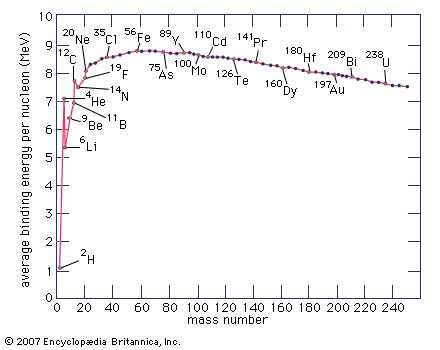
\includegraphics[width=0.5\textwidth]{bindinges}
\end{center}

This curve has a number of interesting features.
\begin{itemize}
  \item There are pronounced peaks at $ w = 4, 12, \text{ and } 16 $. These represent more tightly bound
        nuclei, and are due to filled \textit{nuclear shells} (similar to electron shells).
  \item The binding energy per nucleon becomes roughly constant at around \SI{8}{\mega\electronvolt}, which
        suggests the binding force is only short-range (adding more nucleons around the outside affects the ones
        inside only slightly).
  \item There is a global maximum at around $ w = 60 $, which shows that larger nuclei become more stable by
        breaking up, while smaller nuclei become more stable by fusing together.
\end{itemize}

\subsection*{Decay Revision}
Alpha decay:
\begin{displaymath}
  ^w_n X \rightarrow ^{w - 4}_{n - 2} Y + \alpha + \text{ energy}
\end{displaymath}
where $ \alpha = ^4_2\mathrm{He} $.

Beta-minus (electron) decay:
\begin{displaymath}
  ^w_n X \rightarrow ^{w}_{n + 1} Y + \beta^- + \text{ energy}
\end{displaymath}
where $ \beta^- = e^- $.

Beta-plus (positron) decay:
\begin{displaymath}
  ^w_n X \rightarrow ^{w}_{n - 1} Y + \beta^+ + \text{ energy}
\end{displaymath}
where $ \beta^- = e^+ $.

Gamma decay: the release of a photon ($\gamma$) when a nucleon jumps from a higher to a lower energy state.

\clearpage
\subsection*{Questions}
Useful data: $ c \approx \SI{2.99e8}{\metre\per\second} $, $ h \approx \SI{6.63e-34}{\joule\second} $,
$ e \approx \SI{1.6e-19}{\coulomb} $, $ \SI{1}{\electronvolt} \approx \SI{1.6e-19}{\joule} $, $ \SI{1}{\amu} \approx \SI{1.661e-27}{\kilo\gram} $,
$ m_\text{proton} = \SI{1.007283}{\amu} $, $ m_\text{neutron} = \SI{1.008665}{\amu} $.

\begin{questions}
  \question Show that $ \SI{1}{\amu} \equiv \SI{931.49}{\mega\electronvolt} $.
  \question Consider two nuclei, one of weight \SI{200}{\amu} and one of weight \SI{60}{\amu}.
    \begin{parts}
      \item Which has the higher binding energy? Explain.
      \item Which is more tightly bound? Explain.
    \end{parts}
  \question Calculate the binding energy of $ ^{56}_{30}\mathrm{Fe} $, if $ m(^{56}_{30}\mathrm{Fe}) = \SI{55.9349}{\amu} $.
  \question Calculate, in \si{\mega\electronvolt}, the binding energy per nucleon of $ ^3\mathrm{H} $ and of $ ^2\mathrm{H} $.
            Which is more tightly bound?
  \question
    \begin{parts}
      \item Younger stars contain a lot of hydrogen gas. How do they generate so much energy?
      \item Older stars are richer in helium than hydrogen. Why do they produce less energy than younger stars?
    \end{parts}
  \question Consider $ ^{15}_{8}\mathrm{O} $. If this particle decays via positron emission, what daughter
            particle will be produced and what will the maximum kinetic energy of the released positron be?
  \question The uranium isotope $ ^{238}\mathrm{U} $ undergoes $ \alpha$-decay to $ ^{234}\mathrm{Th} $. What
            is the kinetic energy of the released alpha particle, in \si{\mega\electronvolt}?
  \question Hayden Leete is trying to convert a wooden table into electricity to fuel a nuclear missile. Given
            that the table is \SI{50}{\kg}, and that wood is approximately 50\% water and 50\% carbon by mass,
            how much energy would be released if the table's nuclei were totally split?
  \question The following reaction takes place within a conventional nuclear weapon.
            \begin{displaymath}
              ^{235}_{92}\mathrm{U} + ^1_0\mathrm{n} \rightarrow ^{89}_{36}\mathrm{Kr} + ^{144}_{56}\mathrm{Ba} + 2\left(^{1}_0\mathrm{n}\right)
            \end{displaymath}
            How much energy is released in this reaction?
  \fullwidth{The following two questions are taken from Q25 of the 2016 VUW Scholarship Physics booklet.}
  \question A $ ^{66}_{28}\mathrm{Ni} $ nucleus with a mass of \SI{65.9291}{\amu} decays by $ \beta^- $ emission.
    \begin{parts}
      \part Identify the nucleus that results from this decay.
      \part If the daughter nucleus has a mass of \SI{65.9289}{\amu}, what is the maximum kinetic energy of the emitted $ \beta^- $ particle?
      \part Why would the emitted particle have less than this kinetic energy?
    \end{parts}
  \question
    \begin{parts}
      \part Consider the following nuclear process, in which a proton is removed from an oxygen nucleus.
            \begin{displaymath}
              ^{16}_8\mathrm{O} + \text{ energy } \rightarrow ^{15}_{7}\mathrm{N} + ^1_1\mathrm{p}
            \end{displaymath}
            Find the energy required for this process to occur.
      \part Now, consider a process in which a neutron is removed.
            \begin{displaymath}
              ^{16}_8\mathrm{O} + \text{ energy } \rightarrow ^{15}_{8}\mathrm{O} + ^1_0\mathrm{n}
            \end{displaymath}
            Find the energy required for this process to occur.
      \part Which particle is more tightly bound to the oxygen nucleus? Explain your answer.
    \end{parts}
\end{questions}

\end{document}
